The action of $G=\operatorname{SL}_2(\mathbb R)$ gives a way to move points of $\mathbb H$. We now seek lengths and areas for which these motions preserve geometry. Ordinary Euclidean length does not work: $a(y)$ acts by dilation and changes it by a factor of $y$. To compensate, the length assigned to a tangent vector must depend on its height.

A Riemannian metric specifies a positive-definite symmetric real inner product on each tangent plane, varying smoothly with the point. Here $T_z\mathbb H\simeq\mathbb C$ is viewed as a real vector space. Write a candidate inner product as $B_z(v,w)$. Requiring the action to preserve it means
\begin{equation}\label{eq:metric-invariance}
 B_{gz}\bigl(g'(z)v,g'(z)w\bigr)=B_z(v,w)
 \qquad(g\in G).
\end{equation}
The stabilizer of $i$ acts on $T_i\mathbb H$ by all rotations, so this requirement already determines the inner product there up to scale. Transitivity will then determine it everywhere.

\begin{proposition}[The invariant metric]\label{hyperbolic.invariant-geometry}
Every $G$-invariant Riemannian metric on $\mathbb H$ has the form
\[
 ds^2=\lambda\frac{dx^2+dy^2}{y^2},\qquad \lambda>0.
\]
Its induced Riemannian area is $\lambda\,dx\,dy/y^2$. Conversely, each of these metrics is $G$-invariant.
\end{proposition}

\begin{proof}
We first prove existence of the invariant metrics. Fix $\lambda>0$ and define
\[
 B_z(v,w)=\frac{\lambda}{y^2}\operatorname{Re}(v\overline w),
 \qquad z=x+iy,\quad v,w\in T_z\mathbb H\simeq\mathbb C.
\]
This is a smooth positive-definite symmetric real inner product. To check invariance, let $g=\begin{smallpmatrix}a&b\\c&d\end{smallpmatrix}\in G$. The Möbius derivative formula in \eqref{eq:mobius-identities} and the imaginary-part formula \eqref{eq:mobius-imaginary-part} give
\[
 g'(z)=\frac1{(cz+d)^2},\qquad
 \operatorname{Im}(gz)=\frac{y}{|cz+d|^2}.
\]
For any complex scalar $\alpha$ and complex vectors $v,w$, we have
$\operatorname{Re}(\alpha v\overline{\alpha w})=|\alpha|^2\operatorname{Re}(v\overline w)$. Use this identity with $\alpha=g'(z)$ to obtain
\[
 \begin{aligned}
 B_{gz}\bigl(g'(z)v,g'(z)w\bigr)
 &=\frac{\lambda|g'(z)|^2}{(\operatorname{Im}gz)^2}
       \operatorname{Re}(v\overline w)\\
 &=\frac{\lambda|cz+d|^{-4}}{y^2|cz+d|^{-4}}
       \operatorname{Re}(v\overline w)
 =B_z(v,w).
 \end{aligned}
\]
This proves existence. The coordinate directions are perpendicular, and each Euclidean length is scaled by $\sqrt\lambda/y$. Their area is therefore scaled by $\lambda/y^2$, giving the asserted induced area. Equivalently, the area density is the square root of the determinant of the metric coefficient matrix $\lambda y^{-2}I_2$.

We next prove uniqueness of the invariant metric, beginning at the point $i$. Let $B$ be any invariant Riemannian metric. Set $g=k(\pi/4)$ and $z=i$ in the metric invariance identity \eqref{eq:metric-invariance}. This matrix fixes $i$, and its derivative there is multiplication by $i$, by the stabilizer derivative formula \eqref{eq:stabilizer-derivative}. Thus
\[
 B_i(iv,iw)=B_i(v,w)\qquad(v,w\in T_i\mathbb H).
\]
Taking $v=w=1$ gives $B_i(i,i)=B_i(1,1)$. Taking $v=1$ and $w=i$ gives
\[
 B_i(1,i)=B_i(i,-1)=-B_i(i,1)=-B_i(1,i),
\]
where the last two equalities use real bilinearity and symmetry, respectively. Hence $B_i(1,i)=B_i(i,1)=0$. Put $\lambda=B_i(1,1)>0$.

To compute the inner product of arbitrary vectors, write
\[
 v=\operatorname{Re}(v)\,1+\operatorname{Im}(v)\,i,
 \qquad w=\operatorname{Re}(w)\,1+\operatorname{Im}(w)\,i.
\]
All four coefficients are real, so real bilinearity gives
\[
 \begin{aligned}
 B_i(v,w)
 &=\operatorname{Re}(v)\operatorname{Re}(w)B_i(1,1)
   +\operatorname{Re}(v)\operatorname{Im}(w)B_i(1,i)\\
 &\quad+\operatorname{Im}(v)\operatorname{Re}(w)B_i(i,1)
   +\operatorname{Im}(v)\operatorname{Im}(w)B_i(i,i)\\
 &=\lambda\bigl(\operatorname{Re}(v)\operatorname{Re}(w)
                 +\operatorname{Im}(v)\operatorname{Im}(w)\bigr)
 =\lambda\operatorname{Re}(v\overline w).
 \end{aligned}
\]
Thus the metric at $i$ is the Euclidean inner product multiplied by $\lambda$.

We now transport this calculation to an arbitrary point $z=x+iy$. Keep $z$ fixed and let $\zeta\in\mathbb H$ denote a variable point. The transformation $s(z)=n(x)a(y)$ acts by
\[
 s(z)\cdot\zeta=x+y\zeta.
\]
It sends $i$ to $z$ and has derivative $y$ at $i$. Apply the metric invariance identity \eqref{eq:metric-invariance} with group element $s(z)$, base point $i$, and tangent vectors $v,w\in T_i\mathbb H$. It reads
\[
 B_{s(z)i}\bigl(s(z)'(i)v,s(z)'(i)w\bigr)=B_i(v,w),
 \quad\text{that is,}\quad B_z(yv,yw)=B_i(v,w).
\]
Using real bilinearity on the left and the formula at $i$ on the right gives
\[
 y^2 B_z(v,w)=\lambda\operatorname{Re}(v\overline w),
 \qquad B_z(v,w)=\frac{\lambda}{y^2}\operatorname{Re}(v\overline w).
\]
Here the tangent planes are identified with $\mathbb C$ in our fixed coordinates. Since $z$ was arbitrary, this proves uniqueness everywhere.
\end{proof}

\begin{proposition}[Invariant measures with smooth densities]\label{hyperbolic.invariant-density}
Every $G$-invariant measure with a smooth positive density relative to Lebesgue area has the form
\[
 d\nu(z)=C\frac{dx\,dy}{y^2},\qquad C>0.
\]
Conversely, each of these measures is $G$-invariant.
\end{proposition}

\begin{proof}
Write $d\nu(z)=\rho(z)\,dx\,dy$ with $\rho$ smooth and positive. A holomorphic map has real Jacobian $|g'(z)|^2$, so the change-of-variables formula makes invariance equivalent to
\[
 \rho(gz)|g'(z)|^2=\rho(z).
\]
Equality of measures first gives equality almost everywhere; continuity of both densities makes it hold everywhere. Apply this at $i$ to $s(x+iy)$, whose derivative is $y$. Then $\rho(x+iy)y^2=\rho(i)$, so $\rho(x+iy)=C/y^2$ with $C=\rho(i)>0$. Conversely, the cancellation used in the \hyperref[hyperbolic.invariant-geometry]{metric proof} gives
\[
 \frac{C}{(\operatorname{Im}gz)^2}|g'(z)|^2=\frac{C}{y^2}.
\]
Change of variables therefore proves invariance of every measure with the asserted density.
\end{proof}

We fix the remaining scale by requiring the real tangent vector $1\in T_i\mathbb H$ to have length one. Thus $\lambda=1$, and the metric agrees with the Euclidean metric at $i$. We use its induced area, which fixes $C=1$ as well. If the metric were multiplied by $\lambda$, lengths and distances would be multiplied by $\sqrt\lambda$, whereas area would be multiplied by $\lambda$.

\begin{definition}[Hyperbolic length, distance, and area]\label{hyperbolic.metric}
With this normalization, the hyperbolic metric and its area measure are
\begin{equation}\label{eq:half-plane-metric-area}
 ds^2=\frac{dx^2+dy^2}{y^2},\qquad d\mu(z)=\frac{dx\,dy}{y^2}.
\end{equation}
Here $dx\,dy$ is ordinary Lebesgue area. The real inner product and norm on the tangent plane are
\[
 \langle v,w\rangle_{T_z\mathbb H}
 =\frac{\operatorname{Re}(v\overline w)}{(\operatorname{Im}z)^2},
 \qquad \|v\|_{T_z\mathbb H}=\frac{|v|}{\operatorname{Im}z}.
\]
The notation $ds^2$ records squared infinitesimal length. Along a piecewise continuously differentiable path $\alpha:[a,b]\to\mathbb H$, write $\alpha(t)=x(t)+iy(t)$. Substituting $dx=x'(t)\,dt$ and $dy=y'(t)\,dt$ into the metric gives
\[
 ds^2=\frac{x'(t)^2+y'(t)^2}{y(t)^2}\,dt^2.
\]
Thus the speed is the square root of this coefficient:
\[
 \|\alpha'(t)\|_{T_{\alpha(t)}\mathbb H}
 =\frac{\sqrt{x'(t)^2+y'(t)^2}}{y(t)}
 =\frac{|\alpha'(t)|}{\operatorname{Im}\alpha(t)}.
\]
Integrating speed defines the path length
\[
 L(\alpha)=\int_a^b\|\alpha'(t)\|_{T_{\alpha(t)}\mathbb H}\,dt
 =\int_a^b\frac{\sqrt{x'(t)^2+y'(t)^2}}{y(t)}\,dt.
\]
The hyperbolic distance $d_{\mathbb H}(z,w)$ is the infimum of these lengths over paths joining $z$ to $w$. A geodesic segment is a length-minimizing arc, parametrized proportionally to length when a parametrization is specified.
\end{definition}

\begin{proposition}[Invariance of metric and measure]\label{hyperbolic.invariance}
Every $g\in G$ preserves hyperbolic lengths, distance, and area.
\end{proposition}

\begin{proof}
First we prove preservation of path lengths. At each point where a path $\alpha$ is differentiable, set $z=\alpha(t)$ and $v=w=\alpha'(t)$ in the metric invariance identity \eqref{eq:metric-invariance} with $\lambda=1$. The chain rule identifies the transformed vector as
\[
 (g\circ\alpha)'(t)=g'(\alpha(t))\alpha'(t).
\]
Consequently,
\[
 \begin{aligned}
 \|(g\circ\alpha)'(t)\|_{T_{g\alpha(t)}\mathbb H}^2
 &=\bigl\langle g'(\alpha(t))\alpha'(t),
                 g'(\alpha(t))\alpha'(t)\bigr\rangle_{T_{g\alpha(t)}\mathbb H}\\
 &=\langle\alpha'(t),\alpha'(t)\rangle_{T_{\alpha(t)}\mathbb H}
 =\|\alpha'(t)\|_{T_{\alpha(t)}\mathbb H}^2.
 \end{aligned}
\]
Taking nonnegative square roots gives equality of speeds; integration over the smooth pieces gives $L(g\circ\alpha)=L(\alpha)$.

Next we prove preservation of distance. Composition with $g$ sends paths from $z$ to $w$ to paths from $gz$ to $gw$ of the same length. Composition with $g^{-1}$ is its inverse, so the two sets of possible path lengths agree. Their infima, and hence the distances, agree.

Finally we prove preservation of area. For a measurable set $E\subset\mathbb H$, change variables from $w$ to $w=gz$. Multiplication by the complex derivative $g'(z)$ scales real area by $|g'(z)|^2$, giving
\[
 \begin{aligned}
 \mu(gE)
 &=\int_E\frac{|g'(z)|^2}{(\operatorname{Im}gz)^2}\,dx\,dy\\
 &=\int_E\frac{|cz+d|^{-4}}{y^2|cz+d|^{-4}}\,dx\,dy
 =\int_E\frac{dx\,dy}{y^2}=\mu(E).
 \end{aligned}
\]
The same change of variables applies to nonnegative functions and to integrable functions. The density and Jacobian factors cancel exactly, as required.
\end{proof}

\begin{lemma}[Vertical geodesics and their lengths]\label{hyperbolic.vertical-geodesics}
For $y_1,y_2>0$, the vertical interval from $iy_1$ to $iy_2$ is the unique minimizing arc, and $d_{\mathbb H}(iy_1,iy_2)=|\log(y_2/y_1)|$. Horizontal translation gives the same conclusion on any vertical line.
\end{lemma}

\begin{proof}
Begin with endpoints $iy_1,iy_2$, where $y_1,y_2>0$. Any competing path has the form $\alpha(t)=x(t)+iy(t)$, and its length satisfies
\[
 \begin{aligned}
 L(\alpha)
 &=\int_a^b\frac{\sqrt{x'(t)^2+y'(t)^2}}{y(t)}\,dt\\
 &\geq\int_a^b\frac{|y'(t)|}{y(t)}\,dt
 \geq\left|\int_a^b\frac{y'(t)}{y(t)}\,dt\right|
 =|\log(y_2/y_1)|.
 \end{aligned}
\]
The first inequality discards horizontal motion; the second discards any backtracking in height. A monotone vertical path attains both equalities. Conversely, equality in the first inequality forces $x'=0$ on every smooth piece, so $x$ is constant. Equality in the second forces $y'/y$ to have one sign almost everywhere, so $\log y$ is monotone. Thus the vertical interval is the unique minimizing image, and its distance is $|\log(y_2/y_1)|$. A horizontal translation gives the same conclusion on every vertical line.
\end{proof}

\begin{theorem}[Classification of geodesics]\label{hyperbolic.geodesics}
Two distinct points of $\mathbb H$ lie on exactly one vertical line or Euclidean circle with center on the real axis. The arc between them in $\mathbb H$ is their unique geodesic segment as an unparametrized arc. The complete geodesics are the vertical lines and the upper semicircles perpendicular to the real axis.
\end{theorem}

\begin{proof}
For points on the same vertical line, the \hyperref[hyperbolic.vertical-geodesics]{vertical-geodesic lemma} gives the unique minimizing segment.

We now determine the circle through two points $z=x_1+iy_1$ and $w=x_2+iy_2$ with $x_1\ne x_2$. A center $r$ on the real axis must be equally distant from $z$ and $w$. Expanding that requirement gives
\[
 (x_1-r)^2+y_1^2=(x_2-r)^2+y_2^2,
 \qquad
 2r(x_2-x_1)=x_2^2+y_2^2-x_1^2-y_1^2.
\]
Therefore there is exactly one such center,
\[
 r=\frac{x_2^2+y_2^2-x_1^2-y_1^2}{2(x_2-x_1)}.
\]
Geometrically, $r$ is the intersection of the real axis with the Euclidean perpendicular bisector of the chord joining $z$ to $w$. Put $R=|z-r|=|w-r|$ and $r_1=r-R$, $r_2=r+R$. These are the two real endpoints of the semicircle; \hyperref[hyperbolic.geodesics-diagram]{the diagram below} shows the construction and its vertical image. If instead $x_1=x_2$, distinct points have different heights, and the equal-distance equation has no real solution: their required curve is the vertical line already treated.

\begin{figure}[htbp]
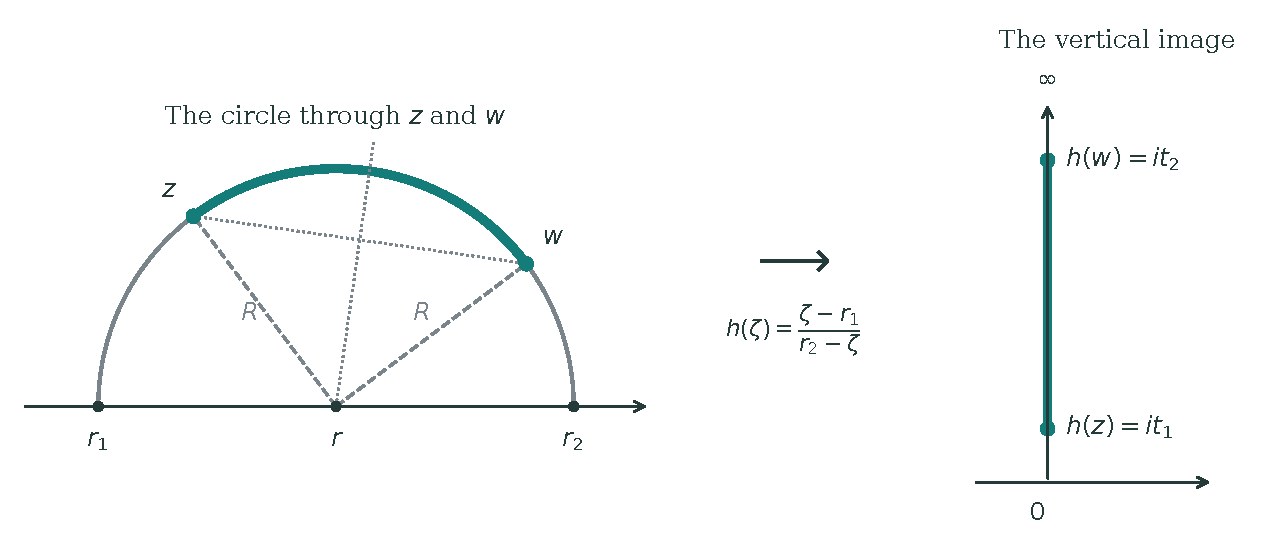
\includegraphics[width=\linewidth]{volumes/Volume01/A/chapters/Chapter01/sections/Section03/figures/geodesics.pdf}
\caption{The center $r$ lies on the real axis and the perpendicular bisector of the chord $zw$; the dashed radii have equal length $R$. The map $h$ sends the semicircle to the positive imaginary axis, carrying its highlighted arc to the highlighted vertical interval and preserving hyperbolic length. The endpoints $r_1,r_2$ go to $0,\infty$, respectively.}
\label{hyperbolic.geodesics-diagram}
\end{figure}

Next we straighten this semicircle. Define, for a variable point $\zeta\in\mathbb H$,
\[
 h(\zeta)=\frac{\zeta-r_1}{r_2-\zeta}.
\]
Its matrix $\begin{smallpmatrix}1&-r_1\\-1&r_2\end{smallpmatrix}$ has positive determinant $r_2-r_1$. Dividing the matrix by $\sqrt{r_2-r_1}$ represents the same transformation by an element of $G$. Thus $h$ is a bijection of $\mathbb H$ preserving lengths. For $\zeta=u+iv$ on our semicircle, the circle equation is equivalent to
\[
 (u-r_1)(r_2-u)=v^2.
\]
Multiplying the fraction defining $h$ by the conjugate denominator now gives
\[
 \begin{aligned}
 \operatorname{Re}h(\zeta)
 &=\frac{(u-r_1)(r_2-u)-v^2}{(r_2-u)^2+v^2}=0,\\
 \operatorname{Im}h(\zeta)
 &=\frac{v(r_2-r_1)}{(r_2-u)^2+v^2}>0.
 \end{aligned}
\]
The image is exactly the positive imaginary axis. Indeed, solving $h(\zeta)=it$ gives
\[
 h^{-1}(it)=\frac{r_1+it r_2}{1+it},\qquad t>0,
\]
Writing this inverse as $u+iv$ and using $r_1=r-R$, $r_2=r+R$ gives
\[
 u-r=\frac{R(t^2-1)}{1+t^2},\qquad v=\frac{2Rt}{1+t^2}>0.
\]
Thus $(u-r)^2+v^2=R^2$, because $(t^2-1)^2+4t^2=(1+t^2)^2$. As $t$ runs from $0$ to $\infty$, this traces the whole upper semicircle. In particular $h(z)=it_1$ and $h(w)=it_2$ for uniquely determined $t_1,t_2>0$.

Every path from $z$ to $w$ now maps to a path from $it_1$ to $it_2$ with the same length. By the \hyperref[hyperbolic.vertical-geodesics]{vertical-geodesic lemma}, the vertical interval is the unique minimizing image between these transformed endpoints, so its inverse image is the unique minimizing circular arc between the original endpoints. Its length is
\[
 d_{\mathbb H}(z,w)=|\log(t_2/t_1)|.
\]
Thus the circle case has been reduced to the vertical case without trying to integrate along a circular parametrization.

The resulting arcs extend to the stated complete geodesics. Conversely, a locally minimizing regular curve must locally agree with one of the unique segments just constructed. At a point, a vertical tangent determines the vertical line; a nonvertical tangent determines a unique real center, since the radius must be perpendicular to that tangent. Hence successive local segments belong to the same circle or line. The vertical parametrization $ie^t$, $t\in\mathbb R$, and its inverse images under $G$ extend these geodesics for all arclength parameters.
\end{proof}

\begin{proposition}[The hyperbolic distance formula]\label{hyperbolic.distance-formula}
For $z,w\in\mathbb H$,
\begin{equation}\label{eq:hyperbolic-distance}
 \cosh\bigl(d_{\mathbb H}(z,w)\bigr)
 =1+\frac{|z-w|^2}{2\operatorname{Im}z\operatorname{Im}w}.
\end{equation}
\end{proposition}

\begin{proof}
We express the distance directly in terms of the endpoints $z,w$. Introduce the temporary quantity
\[
 J(z,w)=\frac{|z-w|^2}{\operatorname{Im}z\operatorname{Im}w}.
\]
For $g=\begin{smallpmatrix}a&b\\c&d\end{smallpmatrix}\in G$, the difference and imaginary-part identities give
\[
 |gz-gw|^2=\frac{|z-w|^2}{|cz+d|^2|cw+d|^2},\qquad
 (\operatorname{Im}gz)(\operatorname{Im}gw)
 =\frac{(\operatorname{Im}z)(\operatorname{Im}w)}{|cz+d|^2|cw+d|^2}.
\]
Dividing proves $J(gz,gw)=J(z,w)$. For distinct endpoints, use the transformation in the \hyperref[hyperbolic.geodesics]{geodesic classification}, or a translation in the vertical case, so that the endpoints become $it_1,it_2$. Both distance and $J$ are preserved. The \hyperref[hyperbolic.vertical-geodesics]{vertical distance formula} gives $d_{\mathbb H}(it_1,it_2)=|\log(t_2/t_1)|$. On that axis,
\[
 \begin{aligned}
 1+\frac{J(it_1,it_2)}2
 &=1+\frac{(t_1-t_2)^2}{2t_1t_2}
 =\frac12\left(\frac{t_2}{t_1}+\frac{t_1}{t_2}\right)\\
 &=\cosh\bigl(\log(t_2/t_1)\bigr)
 =\cosh|\log(t_2/t_1)|.
 \end{aligned}
\]
The final equality uses that $\cosh$ is even. Returning to the original points gives
\[
 \cosh\bigl(d_{\mathbb H}(z,w)\bigr)
 =\cosh\bigl(d_{\mathbb H}(it_1,it_2)\bigr)
 =1+\frac{J(it_1,it_2)}2
 =1+\frac{J(z,w)}2.
\]
Since $\cosh$ is strictly increasing on $[0,\infty)$, this determines the nonnegative distance. For $z=w$ the same formula is immediate from the constant path. For distinct points it gives positive distance; symmetry and the triangle inequality follow from path reversal and concatenation.
\end{proof}

\begin{example}[Unit speed and logarithmic height]\label{hyperbolic.vertical-flow}
Parametrize the vertical geodesic by
\[
 \alpha(t)=ie^t=a(e^t)i,\qquad t\in\mathbb R.
\]
Its height is $\operatorname{Im}\alpha(t)=e^t$, and its velocity is $\alpha'(t)=ie^t$. Hyperbolic speed is Euclidean speed divided by the current height, so
\[
 \|\alpha'(t)\|_{T_{\alpha(t)}\mathbb H}
 =\frac{|ie^t|}{e^t}=1.
\]
Thus the curve has unit hyperbolic speed: increasing the parameter by one traverses an arc of hyperbolic length one. Its Euclidean speed increases with height, but the factor $1/y$ in the metric compensates exactly. The \hyperref[hyperbolic.vertical-geodesics]{vertical distance formula} makes the role of the parameter explicit:
\[
 d_{\mathbb H}(\alpha(t_1),\alpha(t_2))
 =\left|\log\frac{e^{t_2}}{e^{t_1}}\right|
 =|t_2-t_1|.
\]
In particular, changing $t$ to $t+s$ multiplies height by $e^s$ and moves distance $|s|$ along the geodesic. This is why logarithmic height, $t=\log y$, is an arclength coordinate.

The same construction parametrizes a semicircular geodesic at unit speed. Such a semicircle meets the real axis perpendicularly. Let $h$ be the M\"obius transformation from the \hyperref[hyperbolic.geodesics]{geodesic classification proof} that sends it to the positive imaginary axis. Then
\[
 \gamma(t)=h^{-1}(ie^t)
\]
runs along the semicircle with unit hyperbolic speed, since $h^{-1}$ preserves tangent lengths. It also satisfies $d_{\mathbb H}(\gamma(t_1),\gamma(t_2))=|t_2-t_1|$. Thus multiplying height by $e^s$ on the vertical axis becomes a motion through distance $|s|$ along the semicircle after applying $h^{-1}$; the speed here is measured in the hyperbolic metric.

For comparison, fix $y>0$ and parametrize the horizontal segment by $\beta(t)=x_1+t(x_2-x_1)+iy$, $0\leq t\leq1$. Its speed is $|x_2-x_1|/y$, so
\begin{equation}\label{eq:horizontal-segment-length}
 L(\beta)=\int_0^1\frac{|x_2-x_1|}{y}\,dt
 =\frac{|x_2-x_1|}{y}.
\end{equation}
Except for coincident endpoints this segment is not a geodesic, by the classification above.
\end{example}

The same metric also determines a differential operator on functions. We derive it from gradient and divergence so that its coordinate formula follows from the geometry.

\phantomsection\label{hyperbolic.gradient}
For a real-valued $C^1$ function $f$, the gradient $\operatorname{grad}_{\mathbb H}f$ is characterized by
\begin{equation}\label{eq:gradient-characterization}
 \langle\operatorname{grad}_{\mathbb H}f,V\rangle_{T_z\mathbb H}=df_z(V)
 \qquad(V\in T_z\mathbb H).
\end{equation}
Write $V=P\partial_x+Q\partial_y$ and $\operatorname{grad}_{\mathbb H}f=A\partial_x+B\partial_y$. The defining equality becomes
\[
 \frac{AP+BQ}{y^2}=f_xP+f_yQ\qquad\text{for all real }P,Q,
\]
so
\begin{equation}\label{eq:gradient-coordinates}
 \operatorname{grad}_{\mathbb H}f=y^2 f_x\partial_x+y^2 f_y\partial_y.
\end{equation}
The factor $y^2$ is forced by the inner product: it compensates for the $y^{-2}$ in the metric.

\phantomsection\label{hyperbolic.divergence}
Divergence also has a characterizing identity. The gradient is determined by the tangent inner product; divergence is determined by integration by parts with respect to the area measure $\mu$. For a real $C^1$ vector field $V$, define $\operatorname{div}_{\mathbb H}V$ to be the unique continuous real-valued function satisfying
\begin{equation}\label{eq:divergence-characterization}
 \int_{\mathbb H}\phi\operatorname{div}_{\mathbb H}V\,d\mu
 =-\int_{\mathbb H}
   \langle\operatorname{grad}_{\mathbb H}\phi,V\rangle_{T_z\mathbb H}\,d\mu
 \qquad\bigl(\phi\in C_c^\infty(\mathbb H;\mathbb R)\bigr).
\end{equation}
Here the test functions $\phi$ are smooth real functions that vanish outside a compact subset of $\mathbb H$. By the characterizing identity for the gradient \eqref{eq:gradient-characterization}, the inner product on the right is $d\phi(V)$, the directional derivative of $\phi$ along $V$. Thus the identity transfers differentiation from the test function to the vector field, with a minus sign, just as in ordinary integration by parts. Compact support removes boundary terms; the vector field itself need not have compact support.

We now prove that this definition determines a function and derive its coordinate formula. Write $V=P\partial_x+Q\partial_y$ and use $d\mu=y^{-2}\,dx\,dy$. Since $d\phi(V)=P\phi_x+Q\phi_y$, ordinary integration by parts in each coordinate gives
\[
 \begin{aligned}
 -\int_{\mathbb H}d\phi(V)\,d\mu
 &=-\int_{\mathbb H}(P\phi_x+Q\phi_y)y^{-2}\,dx\,dy\\
 &=\int_{\mathbb H}\phi\bigl(\partial_x(y^{-2}P)+\partial_y(y^{-2}Q)\bigr)\,dx\,dy\\
 &=\int_{\mathbb H}\phi\,y^2
   \bigl(\partial_x(y^{-2}P)+\partial_y(y^{-2}Q)\bigr)\,d\mu.
 \end{aligned}
\]
In the last line we used $dx\,dy=y^2\,d\mu$. The coefficient of $\phi$ in that integral is continuous and satisfies the defining identity, proving existence. To prove uniqueness, suppose two continuous functions satisfy it. Their difference integrates to zero against every test function. If the difference were positive at some point, continuity would make it positive on a neighborhood. A nonzero nonnegative smooth test function supported in that neighborhood would give a positive integral, a contradiction. Interchanging the two functions rules out a negative difference as well.

Consequently,
\begin{equation}\label{eq:divergence-coordinates}
 \begin{aligned}
 \operatorname{div}_{\mathbb H}V
 &=y^2\bigl(\partial_x(y^{-2}P)+\partial_y(y^{-2}Q)\bigr)\\
 &=y^2\bigl(y^{-2}P_x+y^{-2}Q_y-2y^{-3}Q\bigr)
 =P_x+Q_y-\frac{2Q}{y}.
 \end{aligned}
\end{equation}
The correction $-2Q/y$ comes from differentiating the area density $y^{-2}$. It is therefore the use of hyperbolic area in the characterizing identity that distinguishes this formula from Euclidean divergence.

\begin{definition}[The hyperbolic Laplace--Beltrami operator]\label{hyperbolic.laplacian}
For a real-valued $C^2$ function on $\mathbb H$, define
\[
 \Delta f=-\operatorname{div}_{\mathbb H}\operatorname{grad}_{\mathbb H}f.
\]
We extend this operator complex linearly to complex-valued functions. The minus sign is the nonnegative convention, justified below. In coordinates,
\[
 \Delta f=-y^2(f_{xx}+f_{yy}).
\]
When using $L^2(\mathbb H,\mu)$, we mean complex-valued functions and the inner product
$\langle f,h\rangle_{L^2(\mathbb H,\mu)}=\int_{\mathbb H}f\overline h\,d\mu$, linear in the first argument.
\end{definition}

The coordinate expression follows from the gradient formula \eqref{eq:gradient-coordinates} and the divergence formula \eqref{eq:divergence-coordinates}:
\[
 \begin{aligned}
 \operatorname{div}_{\mathbb H}\operatorname{grad}_{\mathbb H}f
 &=\partial_x(y^2f_x)+\partial_y(y^2f_y)-\frac{2y^2f_y}{y}\\
 &=y^2f_{xx}+2yf_y+y^2f_{yy}-2yf_y
 =y^2(f_{xx}+f_{yy}).
 \end{aligned}
\]
In particular, the absence of a first-order term comes from cancellation between the gradient and the area density.

\begin{theorem}[The Laplacian commutes with isometries]\label{hyperbolic.laplacian-isometries}
Let $F:\mathbb H\to\mathbb H$ be a smooth Riemannian isometry: a smooth diffeomorphism satisfying
\[
 \langle dF_z(v),dF_z(w)\rangle_{T_{F(z)}\mathbb H}
 =\langle v,w\rangle_{T_z\mathbb H}.
\]
Then, for every $f\in C^2(\mathbb H;\mathbb C)$,
\[
 \Delta(f\circ F)=(\Delta f)\circ F.
\]
In particular this holds for $F(z)=g\cdot z$ with $g\in G$.
\end{theorem}

\begin{proof}
We prove the assertion for real $f$ first. The idea is to use the defining integration-by-parts identity: an isometry preserves both the gradient inner products and the area measure appearing in that identity.

First we check preservation of area. At $z=x+iy$, the isometry condition says that $dF_z$ multiplies Euclidean lengths by $\operatorname{Im}F(z)/y$ and preserves angles. It therefore multiplies Euclidean areas by $(\operatorname{Im}F(z)/y)^2$. The density of hyperbolic area at the image point cancels this factor:
\[
 \frac1{(\operatorname{Im}F(z))^2}
 \left(\frac{\operatorname{Im}F(z)}{y}\right)^2
 =\frac1{y^2}.
\]
Change of variables proves that $F$ preserves $\mu$. This reasoning uses unsigned area and applies whether $F$ preserves or reverses orientation.

Next we check how gradients transform. For any real $C^1$ function $u$ and tangent vector $v$ at $z$, the characterizing identity for the gradient \eqref{eq:gradient-characterization} and the chain rule give
\[
 \begin{aligned}
 \langle\operatorname{grad}_{\mathbb H}(u\circ F)(z),v\rangle_{T_z\mathbb H}
 &=d(u\circ F)_z(v)\\
 &=du_{F(z)}(dF_z(v))\\
 &=\langle\operatorname{grad}_{\mathbb H}u(F(z)),dF_z(v)\rangle_{T_{F(z)}\mathbb H}.
 \end{aligned}
\]
To compare vectors in the same tangent plane, use preservation of inner products to rewrite the left side of this equality at $F(z)$. We obtain
\[
 \begin{aligned}
 &\bigl\langle dF_z\bigl(\operatorname{grad}_{\mathbb H}(u\circ F)(z)\bigr),
                  dF_z(v)\bigr\rangle_{T_{F(z)}\mathbb H}\\
 &\qquad=\langle\operatorname{grad}_{\mathbb H}u(F(z)),
                  dF_z(v)\rangle_{T_{F(z)}\mathbb H}
 \qquad(v\in T_z\mathbb H).
 \end{aligned}
\]
The two vectors being compared are the image under $dF_z$ of the gradient of $u\circ F$ at $z$, and the gradient of $u$ at $F(z)$. Because $F$ has a smooth inverse, $dF_z$ is onto: as $v$ varies, $dF_z(v)$ runs through every vector in $T_{F(z)}\mathbb H$. The displayed equality therefore says that these two vectors have the same inner product with every vector in that tangent plane. Their difference is perpendicular to every vector, hence to itself, so it has squared norm zero and must vanish. This proves
\begin{equation}\label{eq:gradient-transport}
 dF_z\bigl(\operatorname{grad}_{\mathbb H}(u\circ F)(z)\bigr)
 =\operatorname{grad}_{\mathbb H}u(F(z)).
\end{equation}

Now fix $\phi\in C_c^\infty(\mathbb H;\mathbb R)$. We use the transformation law for gradients \eqref{eq:gradient-transport} twice: first with $u=\phi$, then with $u=f$. Preservation of inner products, followed by these two substitutions, gives
\begin{equation}\label{eq:gradient-pairing-transport}
 \begin{aligned}
 &\langle\operatorname{grad}_{\mathbb H}(\phi\circ F)(z),
          \operatorname{grad}_{\mathbb H}(f\circ F)(z)\rangle_{T_z\mathbb H}\\
 &\quad=\bigl\langle dF_z\bigl(\operatorname{grad}_{\mathbb H}(\phi\circ F)(z)\bigr),
                    dF_z\bigl(\operatorname{grad}_{\mathbb H}(f\circ F)(z)\bigr)
          \bigr\rangle_{T_{F(z)}\mathbb H}\\
 &\quad=\langle\operatorname{grad}_{\mathbb H}\phi(F(z)),
                \operatorname{grad}_{\mathbb H}f(F(z))\rangle_{T_{F(z)}\mathbb H}.
 \end{aligned}
\end{equation}
This is the pointwise identity that will allow us to change variables from $z$ to $w=F(z)$ in the integral of the gradient inner product.

We now apply integration by parts with this test function. From $\Delta=-\operatorname{div}_{\mathbb H}\operatorname{grad}_{\mathbb H}$ and the characterizing identity for divergence \eqref{eq:divergence-characterization}, we obtain
\[
 \begin{aligned}
 \int_{\mathbb H}(\phi\circ F)\Delta(f\circ F)\,d\mu
 &=\int_{\mathbb H}
   \langle\operatorname{grad}_{\mathbb H}(\phi\circ F),
          \operatorname{grad}_{\mathbb H}(f\circ F)\rangle_{T_z\mathbb H}\,d\mu(z)\\
 &=\int_{\mathbb H}
   \langle\operatorname{grad}_{\mathbb H}\phi,
          \operatorname{grad}_{\mathbb H}f\rangle_{T_w\mathbb H}\,d\mu(w)\\
 &=\int_{\mathbb H}\phi\,\Delta f\,d\mu\\
 &=\int_{\mathbb H}(\phi\circ F)\bigl((\Delta f)\circ F\bigr)\,d\mu.
 \end{aligned}
\]
The second equality uses the identity for gradient inner products \eqref{eq:gradient-pairing-transport} and the change of variables $w=F(z)$; the third uses integration by parts again, and the fourth changes variables back. All test functions have compact support, so there are no boundary terms.

Because $F$ is a diffeomorphism, $\phi\circ F$ ranges over all smooth compactly supported real test functions. Thus the continuous functions $\Delta(f\circ F)$ and $(\Delta f)\circ F$ have equal integrals against every such function. The same uniqueness argument used to define divergence makes them equal pointwise. Applying the real result to the real and imaginary parts of $f$ proves the complex-valued statement.
\end{proof}

\begin{proposition}[Symmetry and nonnegativity]\label{hyperbolic.laplacian-green}
For $f,h\in C_c^\infty(\mathbb H;\mathbb C)$,
\[
 \langle\Delta f,h\rangle_{L^2(\mathbb H,\mu)}
 =\int_{\mathbb H}(f_x\overline{h_x}+f_y\overline{h_y})\,dx\,dy
 =\langle f,\Delta h\rangle_{L^2(\mathbb H,\mu)}.
\]
In particular $\langle\Delta f,f\rangle_{L^2(\mathbb H,\mu)}\geq0$.
\end{proposition}

\begin{proof}
The factor $y^2$ in $\Delta$ cancels the density $y^{-2}$ in $d\mu$, so
\[
 \langle\Delta f,h\rangle_{L^2(\mathbb H,\mu)}
 =-\int_{\mathbb H}(f_{xx}+f_{yy})\overline h\,dx\,dy.
\]
Integrating once by parts in each coordinate gives the middle expression. Integrating once more, now moving the remaining derivative to $h$, gives the last expression. All boundary terms vanish because the supports are compact subsets of the open half-plane. Setting $h=f$ gives the nonnegative integral $\int_{\mathbb H}(|f_x|^2+|f_y|^2)\,dx\,dy$.
\end{proof}

This proposition proves symmetry and nonnegativity on the domain $C_c^\infty(\mathbb H;\mathbb C)$. Self-adjointness is a further assertion about an operator together with its domain: its domain must equal that of its Hilbert-space adjoint. Integration by parts alone does not establish this. We defer the closed realization, its domain and self-adjointness, and the corresponding quotient operators to \hyperref[v1a-ch11]{the spectral chapter}.
